\subsection{Ensemble Toolkit}

An ensemble-based application is a \textbf{workflow}, i.e., a set of tasks
with dependencies that determine the order of their execution. Subsets of
these tasks can be \textbf{workloads}, i.e., tasks whose dependencies have
been satisfied at a particular time and may be executed concurrently.
Ensemble-based application vary in the type of coupling between tasks, the
frequency and volume of exchange between these tasks, and the executable of
each task. This type of applications requires specific coordination,
orchestration and execution protocols, posing both domain-specific and
engineering challenges.

Ensemble Toolkit (EnTK), the topmost layer of RCT, simplifies the process of
creating and executing ensemble-based applications with complex coordination
and communication requirements. EnTK decouples the description of
ensemble-based applications from their execution by separating three orders
of concern: specification of task and resource requirements; resource
selection and acquisition; and execution management. Domain scientist retain
full control of the implementation of their protocols by programming
ensemble-based applications in terms of what should be executed, when and
where. EnTK automates the process of acquiring the resources needed by those
applications and managing their execution via a runtime system like
RADICAL-Pilot.

% A key objective of EnTK is to provide a solution to the execution of
% ensemble-based applications that is independent of the nature of tasks.

EnTK has been used to develop the ExTASY~\cite{balasubramanian2016extasy}
framework for the execution of MD-based advanced sampling methods. EnTK is
also being utilized to develop ensemble-based applications to execute
workflows in the seismology and climate science. Each use case requires
different workflows, with different types of tasks, executed on specific HPC
resources. EnTK supported the development of a simulation-analysis pattern
for ExTASY, implementing two sampling algorithms for execution of both
multithreading and MPI tasks on ARCHER, Stampede and Blue Waters HPC
machines. With the same code base, EnTK is being used to develop inversion of
full-waveform, wide-bandwidth data for seismic tomography, and a new
downscaling methodology to quantify the photovoltaic (PV) energy potential in
selected regions of the USA\@.

Currently, EnTK enables the execution of up to \(O(10^4)\) tasks on thousands
of CPU and GPU nodes on the resources of XSEDE, ORNL, NCSA, NWSC and UK NSS,
for a total of eight HPC machines. At this scale, multiple sources of failure
affect execution, producing loss of information and compute time. Thus, fault
tolerance and recovery capabilities are first order concerns of the design of
EnTK\@. As such, EnTK can handle task execution failures, resource-level
failures, and failures of its own subcomponents and subprocesses, including
network connectivity issues.

EnTK exposes four components to the end-user: `Resource Handle', `Pipeline',
`Stage', and `Task'. These enable users to create ensemble-based applications
and specify target resources for their execution. Internally the `Application
Manager' and `Execution Manager' components enable the acquisition of
resources and the management of application execution (see
\textbf{Figure~\ref{fig:entk_arch}}, right schematic of left panel).

\begin{figure}[!htbp]
  % \centering
  %\begin{minipage}[b]{0.6\textwidth}
  \begin{minipage}[b]{0.49\textwidth}
  \centering
  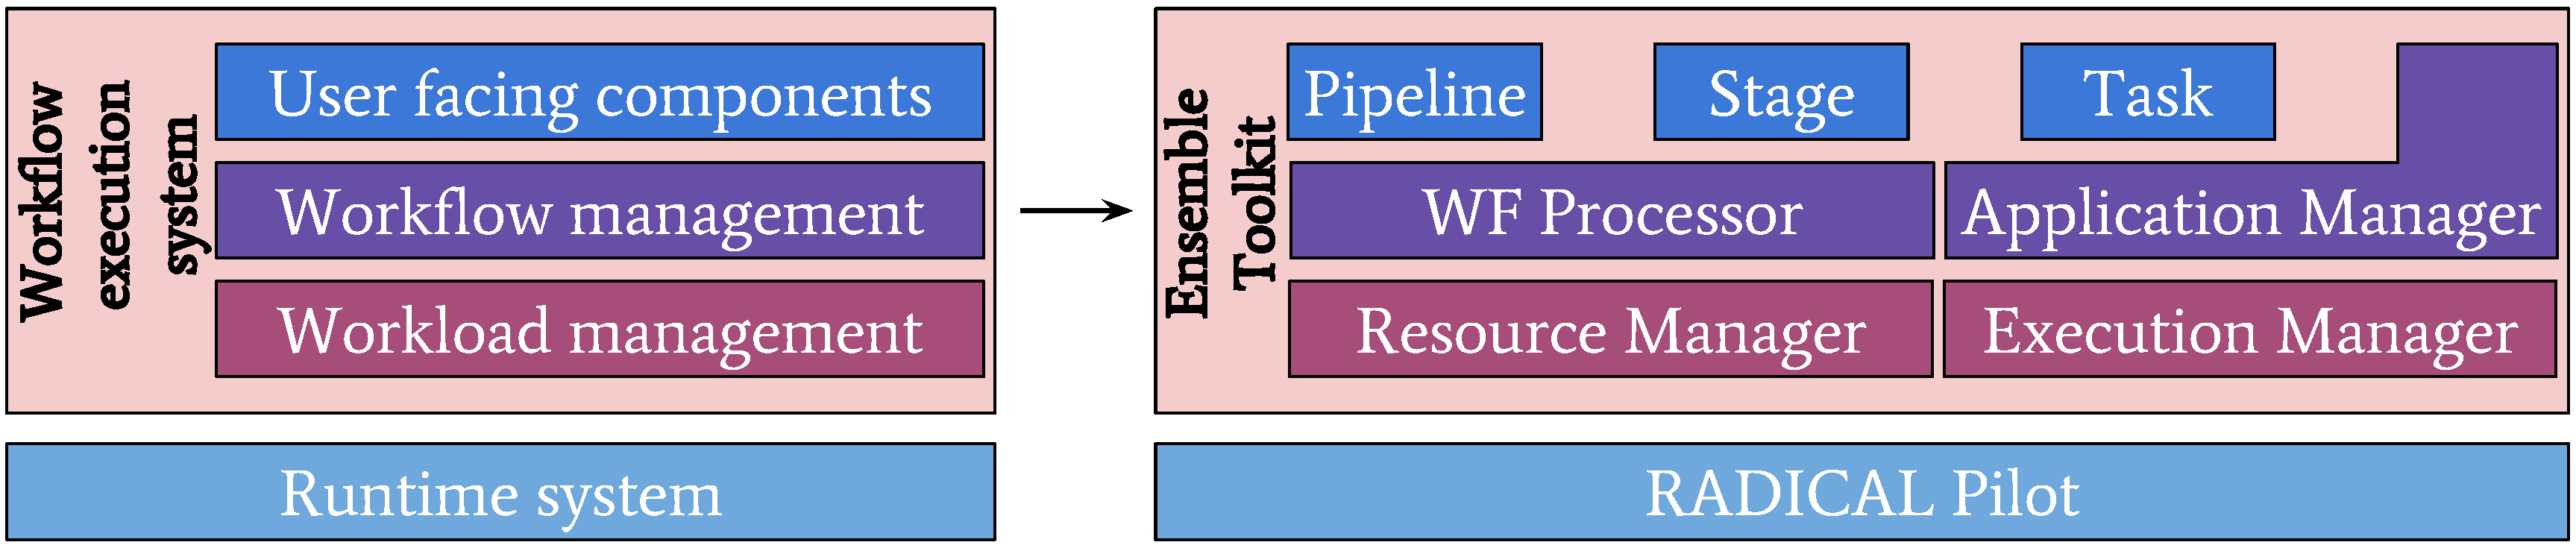
\includegraphics[width=\textwidth]{FIGURES/entk_overview.pdf}
  \end{minipage}
  % \begin{minipage}[b]{0.39\textwidth}
  % \begin{minipage}[b]{0.49\textwidth}
  % \centering
  % \includegraphics[width=\textwidth, height=35mm]{FIGURES/md_general.pdf}
  % \includegraphics[width=\textwidth, height=40mm]{FIGURES/md_general.pdf}
  % \end{minipage}
  \caption{\textbf{Left:} Ensemble Toolkit overview, showing how the abstract
           workflow execution system is mapped to specific components exposed
           to the users and components internal to the toolkit
           % \textbf{Right:} General MD workflow overview that broadly
           % describes the science methods to study the physical
           % systems
           }\label{fig:entk_arch}
\end{figure}

The \textbf{Resource Handle} component is used to describe the set of
resources to be utilized. This includes properties like walltime, number of
nodes, or credentials of resources. The \textbf{Task} component is used to
indicate an executable alongside its input/output data and the requirements
for its executing environment. The \textbf{Stage} component is used to group
tasks that have the same dependencies and can be executed concurrently, while
the \textbf{Pipeline} component is used to describe a sequence of stages,
i.e., stages that need to be executed sequentially, not concurrently.

EnTK enables users to program ensemble-based applications directly in Python,
without requires a domain-specific language. The use of the Task, Stage, and
Pipeline components avoids the need to express explicitly relationship among
tasks. These relationships are insured by design, depending on the
partitioning of the set of tasks into stages and then pipelines. Further,
EnTK enables an explicit definition of pre and post conditions on the
execution of tasks, stages, and pipelines, enabling a fine grained
adaptivity, both a local and global level. Conveniently, this does not
require the codification of a DAG, a process that imposes a rigid
representation model on the domain scientists.

Once the workflow of an ensemble-based application is completely described,
one or more pipelines are submitted to the \textbf{Application Manager}
module for execution. The Application Manager sets up a messaging
infrastructure to enable fault tolerance and then processes each pipeline,
identifying tasks which have their dependencies satisfied and can be executed
concurrently. These tasks are then handed over to the \textbf{Execution
Manager} that binds tasks to resources on the base of a set of
heuristic-based decisions called ``execution strategy''. The Execution Manager
then uses the underlying runtime system, RADICAL-Pilot, to execute the tasks
on the specific target resource.

EnTK is implemented as a multiprocess application. The number of processes
can be tuned to match the throughput requirements of ensemble-based
applications and the capabilities of diverse target resources. All but the
master process of the toolkit are stateless, enabling process-level fault
tolerance. Upon failure of one or more stateless process, application tasks
can be assigned to existing or newly created processes without blocking the
overall execution. Upon failure of the master process, execution can be
restarted without loosing data about tasks that have been already executed.

% Scalability results from an early version of EnTK are provided in
% \textbf{Figure~\ref{fig:entk_perf}}. The number of simulations and the
% total number of cores used are described on the abscissa with each
% simulation using one core; the analysis task which uses one core). Thus,
% the simulation execution time corresponds to the time taken by all the
% simulations to complete.  The analysis execution time corresponds to the
% time taken to analyze the output of all the simulations. Notice how both
% strong and weak scaling up to $O(10^3)$ are linear. Although performance
% numbers are for Stampede (TACC), it is reasonable to expect the weak and
% strong scaling of EnTK to hold firm on Titan as well. The task launching
% and coordination system use the same underlying runtime system --
% RADICAL-Pilot, which has been tested for strong and weak scalability on
% Titan~\cite{angius2017converging} up to $O(10^3)$ tasks. Currently, EnTK
% and RADICAL-Pilot support the execution of ensemble-based applications up
% to $O(10^4)$ tasks. At the next release, planned for Sep 2017, EnTK will
% support $>$ $O(10^4)$ tasks. During the lifetime of this INCITE project
% EnTK is being re-designed, implemented and optimized to reach
% $O(10^5-10^6)$ concurrent tasks, independent of the size and type of task.

% \begin{figure}[!htbp]
% \centering
% \begin{minipage}[b]{.49\textwidth}
%   \centering
  %  \includegraphics[width=\textwidth]{FIGURES/entk_perf_strong.pdf}
  %  \caption{Strong scaling behavior of Ensemble Toolkit. The
  %  total workload is kept constant at 1024 simulations and the amount of
  %  resources used are varied from 64 to 1024. We observe close to linear
  %  drop in the simulation execution time as the amount of resources are
  %  doubled}
% \end{minipage}
% \begin{minipage}[b]{.49\textwidth}
%    \centering
  %  \includegraphics[width=\textwidth]{FIGURES/entk_perf_weak.pdf}
  %  \caption{Weak scaling behavior of Ensemble Toolkit. The size of the
  %  workload is varied in proportion with the amount of resources such that
  %  all tasks are concurrently executed at all times. We observe similar
  %  simulation execution times at all configurations.}
% \end{minipage}
% \caption{\textbf{Left:} Strong scaling of EnTK\@. The total workload is
%         kept constant at 1024 simulations and the resources used are varied
%         from 64 to 1024 cores. We observe essentially linear drop in the
%         simulation execution time. \textbf{Right:} Weak scaling of EnTK.
%         The size of the workload is varied in proportion with the amount of
%         resources such that all tasks are concurrently executed at all
%         times. We observe similar simulation execution times at all
%         configurations.}\label{fig:entk_perf}
% \end{figure}
